\documentclass[a4paper,11pt]{article}
\usepackage{jinstpub}
\usepackage{lineno}
\usepackage[outdir=./]{epstopdf}
\usepackage{multicol}
\usepackage{multirow}
\usepackage{longtable}
\usepackage{array}
\usepackage{rotating}
\usepackage{arydshln}

\usepackage{ptdr-definitions}
\usepackage{custom-definitions}

\usepackage{enumerate}

\graphicspath{
{Figures/}
}

\newcommand{\orc}{
\includegraphics[height=\fontcharht\font`A]{orcidlogo}}
\newcommand{\orcid}[1]{\href{https://orcid.org/#1}{\orc}}
\newcommand{\kernum}[1]{\ensuremath{#1^\prime}\xspace}


\linenumbers


\title{A compact, recurrent, and convolutional neural network decoder for surface codes}

\author{Ula{\c s}can Sar{\i}ca\orcid{0000-0002-1557-4424}}
\affiliation{University of California, Santa Barbara\\Santa Barbara, CA, USA}

\emailAdd{ulascan90@gmail.com}

\abstract{
Current approaches to quantum error decoding include dedicated neural network architectures. They have been shown to outperform algorithmic approaches in accuracy, and come with the potential capability to learn complex qubit readout parameters. Running these architectures on hardware acceleration devices such as FPGAs, GPUs, and other specialized ASICs is needed for fast quantum error correction cycles, so the mathematical representation and number of parameters used in the neural network need to be as compact as possible. In this work, we demonstrate a recurrent, convolutional neural network decoder that can run on surface codes using a compact architecture that exploits the rotational and translational symmetries of the qubit layout. For any distance $d \geq 7$, this compact architecture requires the same, fixed number of less than 100,000 parameters to represent the error states of each round in an error correction cycle, and it features a final decoder layer that scales with $d^2$ to convert the state representation to error predictions on logical observables. Through this representation, we reach error decoding accuracies comparable to some of the other algorithmic approaches in the literature for $d=5$ surface codes, with tests of $d=7$ codes also indicating competitive promise. Together with the inclusion of information from qubit readout, this compact architecture therefore presents itself as a viable option for implementing in hardware acceleration devices in the future.
}



\begin{document}
\maketitle
\flushbottom

\section{Introduction}

Current approaches to quantum error correction (QEC) involve the design of dedicated neural network (NN) architectures to decode errors. These architectures provide potential capability to learn complex qubit readout parameters and error patterns that are difficult to quantify experimentally, and there is evolving expertise to run these NNs on hardware acceleration devices such as FPGAs, GPUs, and other specialized ASICs, which is needed to parallelize the computations and limit the duration of quantum error correction cycles to $\ll 1\mus$. It is estimated that FPGA implementations can potentially reduce delays from QEC cycles below $90\ns$ while dedicated ASICs can further reduce the time to $<30\ns$~\cite{Overwater:2022qwb}.

In another recent study~\cite{Bausch:2023jgi}, NNs running on the Google Sycamore chip have been shown to outperform other techniques based on minimum-weight perfect-matching (MWPM), \eg, PyMatching~\cite{Higgott:2023}, and tensor networks. This study presents a transformer-based recurrent, convolutional neural network architecture that requires slightly over five million trainable NN parameters, and the architecture implements the capability to process flattened qubit I-Q readout inputs to further enhance error detection accuracy.

Running error decoding NNs on FPGAs or dedicated ASICs requires the mathematical operations and the number of parameters used in the NN to be as compact as possible, so the NN architecture needs to be designed carefully. The state-of-the-art FPGAs can typically accept only $\Order(100,000)$ parameters, so NNs with over a million parameters would need a more involved room-temperature computational support system to decode errors in real time, thereby increasing the costs for a commercial quantum computing system.

For this reason, our primary goal in this paper is to outline an alternative approach to design the decoder NN architecture by maximizing the number of NN parameters shared. While our investigation does not yet take additional input from hardware readout into account, we would naively expect only a modest increase in the number of parameters to account for such additional input, likely with a growth factor quadratic in terms of the distance parameter of the QEC code. Since our primary focus has been to find a method to account for the rotational and translational symmetries, we leave a more thorough implementation of accounting for nonuniformities in hardware noise to a future study, providing only a simplistic option in our architecture as an example avenue to explore.

Within these limitations, minimal settings in our NN architecture can reduce the number of parameters to $\leq 72917$ for all surface codes, which is close to a two orders of magnitude improvement with respect to Ref.~\ref{Bausch:2023jgi}, while maintaining decoder performance reaching the levels of PyMatching~\cite{Higgott:2023}. For distance-5 surface codes, our NN decoder is on par with this algorithm in a subset of its operational modes. The code for our compact recursive, convolutional NN (RCNN) architecture can be found in this Github repository~\cite{ourcode} and is based on the TensorFlow Python API~\cite{tensorflow,tensorflow2}.

Throughout the rest of the paper, we will use the following glossary when describing the components of the neural and relating them to a QEC workflow:
\begin{itemize}
\item Round: A single, complete set of stabilizer measurements over the circuit that only leaves logical observables as additional degrees of freedom.
Note that we may occasionally use jargon like ``time-step'' or ``over time'' and the unit of time being used, unless stated otherwise explicitly, is the passage of a round.
\item Cycle: A set of stabilizer measurement rounds upon which either error correction is applied (or errors are tracked) or the data qubits are measured. We will reserve the symbol $r$ to refer to the total number of rounds in a cycle.
\item Kernel distance, $k$: The distance of the underlying surface code that is used in the convolution kernels of the NN architecture. The kernel construct is described in Section~\ref{sec:kernels}, and we will use the value $k=3$ for most of the discussion in this paper.
\item Surface code with distance $d$: When referring to surface codes, we will explicitly refer to rotated surface codes~\cite{Bombin:2007}. While the implementation of our NN architecture assumes this configuration, future investigations could easily account for unrotated surface codes or other structured codes, \eg, the more general class of low-density parity-check codes, using similar concepts.
\item $z$-like variable: A real-valued NN parameter or derived variable that can take values within $(-\infty, \infty)$. For most of the $x$-like, or $p$- and $f$-like variables, described below, that are obtained from an underlying $z$-like value, this $z$-like value is clipped between $\pm12$ in order to avoid singularities in derivatives, which arise fundamentally from the floating-point precision issue $e^z \to 0$ (1) for very small (large) signed values of $z$.
\item $x$-like variable: A real-valued transformed NN variable that can take values within $[0, \infty)$. As done in this paper, one can obtain such values using the transformation $x(z)=e^z$, with the useful property that $x(-z)=1/x(z)$.
\item Sigmoid activation/transformation: There are many options in the literature to transform a $z$-like variable into values bounded asymptotically as $z \to \pm \infty$. When we use this term in this paper, we will explicitly refer to the transformation $\sigma(z)=\left(1+e^{-z}\right)^{-1}$, with the useful property that $\sigma(-z)=1-\sigma(z)$.
\item $p$- (probability) or $f$- (fraction) like variable: A real-valued NN variable that can take values within $(0, 1)$, or $[0,1]$ if the bounds are included explicitly in an embedding parametrization. In the case of exclusive bounds, these variables are obtained using a sigmoid transformation.
\item $c_\varphi$- or $\alpha$-like parameters: A real-valued NN variable that can take values within $(-1, 1)$. These variables can be obtained via a hyperbolic tangent transformation over $z$-like trainable variables. While the way to obtain these parameters are the same, we will distinguish their meaning as the cosine of a phase difference for $c_\varphi$, and a $z$-like variable sign inversion control parameter for $\alpha$.
\item Detectors/detector events: A set of measurements that can be used to flag potential errors. The formalism to define detector events is explained in Refs.~\cite{Gidney:2021,Higgott:2023,Bausch:2023jgi}. One example for detectors would be an XOR of the readouts of the same measure qubits over two consecutive rounds. While stabilizer measurement values are denoted with the reserved letter $m$, detector events are denoted with the reserved letter $e$ throughout this paper, unless it is clear from the context that we are referring to exponentiation using Euler's number.
\end{itemize}

The logical flow of the paper is as follows: In Section~\ref{sec:kernelconstruct}, we describe the kernel concept that maximizes the sharing of NN weights and respects the approximate (exact if hardware noise were uniform) rotational and translational symmetries of the circuit. Section~\ref{sec:kerncomb} is dedicated to the discussion of how the output of kernels is combined, and Section~\ref{sec:rcnn} describes how our kernel concept can be utilized for a recurrent NN architecture. We provide a final summary of our findings and outlook for future investigations in Section~\ref{sec:summary}.


\section{Kernel construction for convolutions}

\subsection{Simple case with $r=2$ error correction cycles}

\subsection{Representation of measure qubit state changes when $r\geq 3$}


%%%%%%%%%%%%%%%%%%%%%%%%%%%%%
\begin{figure*}[htb]
\centering
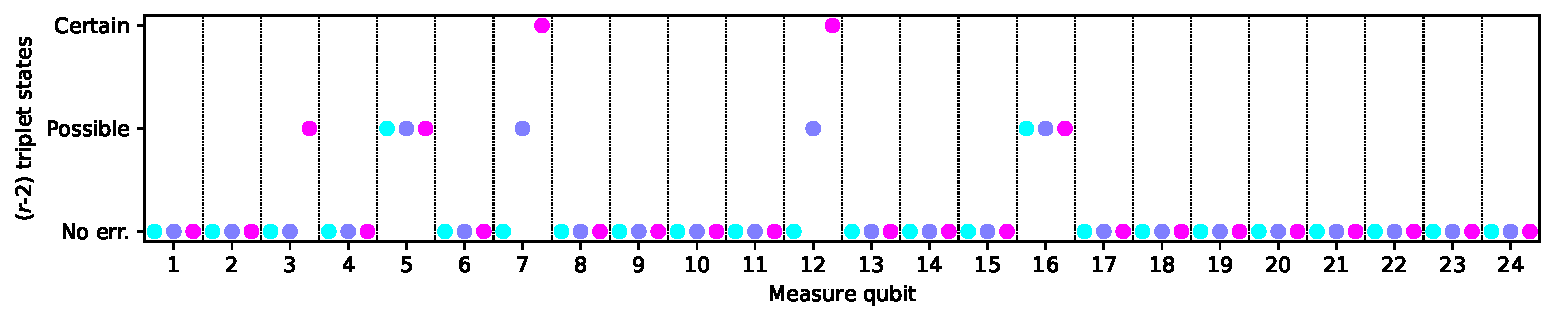
\includegraphics[width=0.9\textwidth]{states_d5_r5_event0.pdf} \\
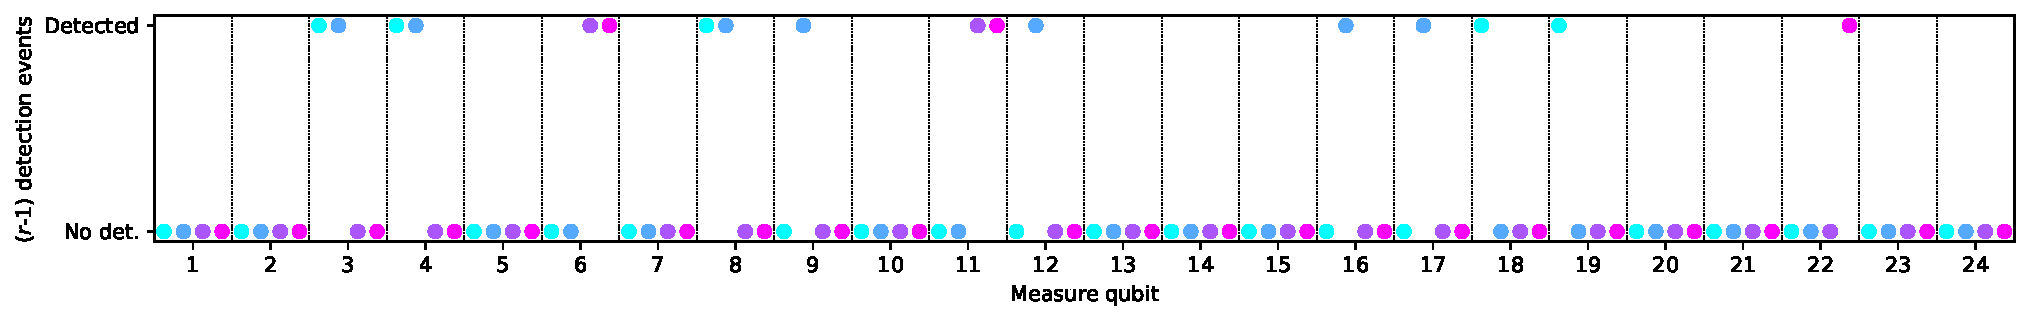
\includegraphics[width=0.9\textwidth]{det_evts_d5_r5_event0.pdf}
\ccaption
{Measure qubit raw states and detection events for $d=5$, $r=5$}
{
}
\label{fig:d5r5states}
\end{figure*}
%%%%%%%%%%%%%%%%%%%%%%%%%%%%%



\subsection{Recurrent convolutional kernel architecture for $r\geq 3$}


\section{Translating kernel outputs as inputs to higher-order layers}

%%%%%%%%%%%%%%%%%%%%%%%%%%%%%
\begin{figure*}[htb]
\centering
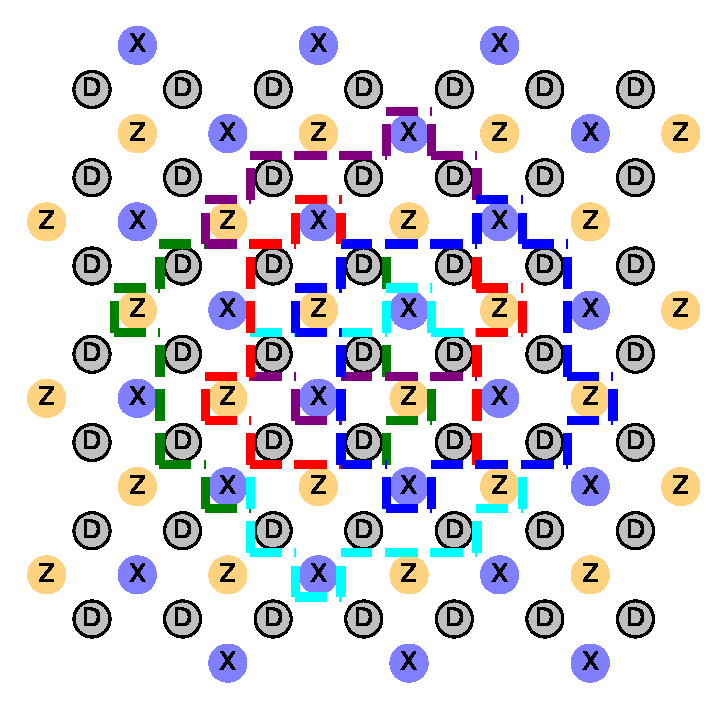
\includegraphics[width=0.6\textwidth]{d7_q25_kernels.pdf}
\ccaption
{$d=3$ kernels surrounding a data qubit in a $d=7$ surface code}
{
}
\label{fig:d7wkern}
\end{figure*}
%%%%%%%%%%%%%%%%%%%%%%%%%%%%%

In the example shown for a $d=7$ code in Fig.~\ref{fig:d7wkern}, all of the displayed kernels are of the same unique type. We highlight the central red kernel as a standard $d=3$ surface code patch and the blue one corresponding to its flipped counterpart. For simplicity, we will number all data qubits from 1 (top left) to 7 (top right) and 49 (bottom right) and denote the corresponding qubit numbers on the kernel patch with a prime indicator, \eg, qubit 18 $\rightarrow$ \kernum{2} in the red kernel and \kernum{3} in the blue one.

Kernels assume uniform noise to maximize the number of weights shared. Symmetries are broken in kernel types that evaluate et the boundary of the surface code. For that reason, all of the weights become unique, and these kernels have 9 outputs. In the only kernel type that does not evaluate at any boundary, only the weights that are associated with kernel qubits \kernum{1}, \kernum{2}, \kernum{3}, \kernum{5}, \kernum{6}, and \kernum{9} are unique, and this kernel has 6 outputs instead of 9.

The kernels displayed in Fig.~\ref{fig:d7wkern} surround qubit 25, the only qubit that can be shared exclusively by kernels of the last type, and we will use this qubit as an example to explain the translation of kernel outputs. Here, the nine kernels colored in red, blue, dark green, magenta, cyan, pink, light green, brown, and orange contribute to the prediction for an error in this qubit with outputs that correspond to kernel qubit positions \kernum{5}, $\kernum{4}\equiv\kernum{6}$, \kernum{6}, $\kernum{8}\equiv\kernum{2}$, \kernum{2}, $\kernum{9}\equiv\kernum{1}$, $\kernum{7}\equiv\kernum{3}$, \kernum{3}, and \kernum{1} respectively. For that reason, these contributions can be encoded as a list of ordered binary integers as $\{(5,1)^2, (5,2)^2, (5,3)^2, (5,5), (5,6)^2\}$, with the first integer in each pair corresponding to the unique type of the contributing kernel, the second one marking the contributing kernel qubit position, and the exponent indicating the number of occurrence of this pair. The number of such unique contributions and the total count of associated parameters are listed in Table~\ref{table:unique-kern-contribs}.

%%%%%%%%%%%%%
\begin{table}[htbp]
\centering
\ccaption
{Parameter counts to combine kernels}
{The counts are listed separately for kernel sizes $k=3$ and $k=5$ over distance-$d$ surface codes. The numbers $C$ refer to the total number of unique combinations of kernel contributions to each of the $d^2$ data qubits. The composition of these combinations determines the number of fraction and phase parameters needed in the NN, with the number of fraction parameters reported for the recursive method described in the main text. For any odd kernel size $k$, parameter counts alternate with the same values for odd and even $d$ above $2k+1$, \ie, 7 for $k=3$ and 11 for $k=5$.}
\renewcommand{\arraystretch}{1.25}
\begin{tabular}{c ccc ccc}
\hline
      & \multicolumn{3}{c}{$k=3$} & \multicolumn{3}{c}{$k=5$} \\
\hline
$d$ & ~~~$C$ & Fractions & Phases & ~~~$C$ & Fractions & Phases  \\
\hline
4 & ~~~4 & 5 & 8 & ~~~- & - & - \\
5 & ~~~13 & 28 & 62 & ~~~- & - & - \\
6 & ~~~9 & 27 & 80 & ~~~9 & 16 & 28 \\
7 & ~~~25 & 86 & 262 & ~~~25 & 88 & 272 \\
8 & ~~~16 & 59 & 182 & ~~~16 & 84 & 400 \\
9 & ~~~25 & 86 & 262 & ~~~41 & 268 & 1504 \\
10 & ~~~16 & 59 & 182 & ~~~25 & 194 & 1272 \\
11 & ~~~25 & 86 & 262 & ~~~61 & 522 & 3554 \\
12 & ~~~16 & 59 & 182 & ~~~36 & 328 & 2282 \\
\hline
\label{table:unique-kern-contribs}
\end{tabular}
\end{table}



If each output of a kernel is bounded between 0 and 1, through sigmoid activation, and can loosely be interpreted as a probability $p_i$ for an error, the combined prediction can be written through the reparametrization $x_i=\sqrt{\frac{p_i}{1-p_i}}$. Using an analogy to write the magnitude of a complex number from a sum of two others, the parameter $x$ for the combined probability can therefore be expressed as
\begin{eqnarray}
S_i &=& \sum_{k_i=1}^{n_i} f_i x^2_{k_i} \\
x^2 &=& \sum_{i=1}^{N} S_i + 2 \sum_{j=i+1}^{N} \sqrt{S_i S_j} \cos{\phi_{ij}}.
\label{eq:kernsum}
\end{eqnarray}
Here, the indices $i$ and $j$ run over a total of $N$ unique contributions, \eg, $N=5$ for qubit 25, and the indices $k_i$ run over $n_i$ different kernel evaluations of the unique combination $i$ of the kernel type and the kernel qubit index, \eg, for contribution type $(5,5)$ to qubit 25, $k_i$ can only be 1, but for all other contribution types it runs from 1 to 2.
The fractions $f_i$ are subject to the constraint $\sum_{i=1}^{N} f_i = 1$, so they can be parametrized using recursive fractions, which would satisfy the constraint by construction and avoid a spurious parameter, \ie, through the mapping $f_1 \to f_1$, $f_i \to f_i\prod_{j=1}^{i-1}\left(1-f_j\right)$ for $1<i<N$, and $f_N \to \prod_{j=1}^{N-1}\left(1-f_j\right)$. Both these fractions and the parameters $\cos{\phi_{ij}}$ are to be handled as unique sets of weights between 0 and 1 to be determined during NN training.

The final probability $p$ computed from the output of all kernels could simply be found from the inverse transformation on $x$, \ie, $p=\frac{x^2}{1+x^2}$, but as a further input to the higher hierarchy of layers, we keep it untransformed as $x^2$. Since there are $d^2$ such values, corresponding to each physical data qubit, leaving $x^2$ as it is adds flexibility for the NN to learn nonuniform noise at the level of higher layers.





\section{Compact RCNN architecture}
\label{sec:rcnn}

The overview of workflow within the RCNN architecture is displayed in Fig.~\ref{fig:RCNN-layout}. After measuring $r$ rounds of stabilizers and translating them to $r+1$ time steps of detector events, the NN redistributes these inputs spatially into the strides of each kernel type and also groups them temporally for the different temporal stages of the architecture. The different temporal stages are shown in Fig.~\ref{fig:RCNN-layer-prog} and are divided as an initial stage, a lead-in stage for recurrence, a true recurrent stage, and a final stage, each handled by their own NN layers and unique sets of parameters. The initial and final layers examine the first and last two rounds of stabilizer measurements, respectively, whereas the lead-in and recurrent layers examine three rounds at a time.

Each of the temporal layers start with the evaluation of all kernel strides, followed by the combination of kernel outputs. All temporal layers share the same base class, and they are differentiated by the nuances in kernel evaluation steps. Except for the initial state kernel, all kernels receive the initial error states of the data qubits that are included in a stride, and the error states from the last round if those are distinct from the initial states. The passed error states are those evaluated from the full temporal layer (denoted with $z^{\,\prime\prime}$ in Fig.~\ref{fig:RCNN-layout}), not the error states from the corresponding kernel strides from previous rounds (denoted with.$x^{\,\prime}$ in Fig.~\ref{fig:RCNN-layout}). While the implementation of the lead-in and recurrent kernel layers is through the same base class in the architecture, we separate them conceptually given that only the recurrent kernel layer can access at least two distinct prior data qubit error states, whereas in the lead-in kernel layer, the output of the initial temporal layer serves as the only unique prior error state that can be passed.

The output of temporal layers is passed through the same decoder layer, which is responsible for decoding the $z$-like error states over the data qubits at each round into the probability of an error over the chosen logical observable (or the probability space over the chosen observables). 
In the current architecture, the decoder layer consists of $d^2$ $z$-like inputs, mapped first to a pair of hidden dense layers with bias parameters and ReLU activation, and then to the output probability space through a sigmoid activation and, again, with a set of bias parameters. For the hidden layers, our tests at $d=5$ suggest 100 nodes to be a reasonable size for each, but rigorous tests for the dependence of the number of hidden layer nodes to $d$ should be performed in future studies. While separate decoder layers could be conceived for each temporal layer type, we have not found any significant improvement in round-by-round and final accuracy levels by constructing independent decoder layers.

\begin{figure*}[htb]
\centering
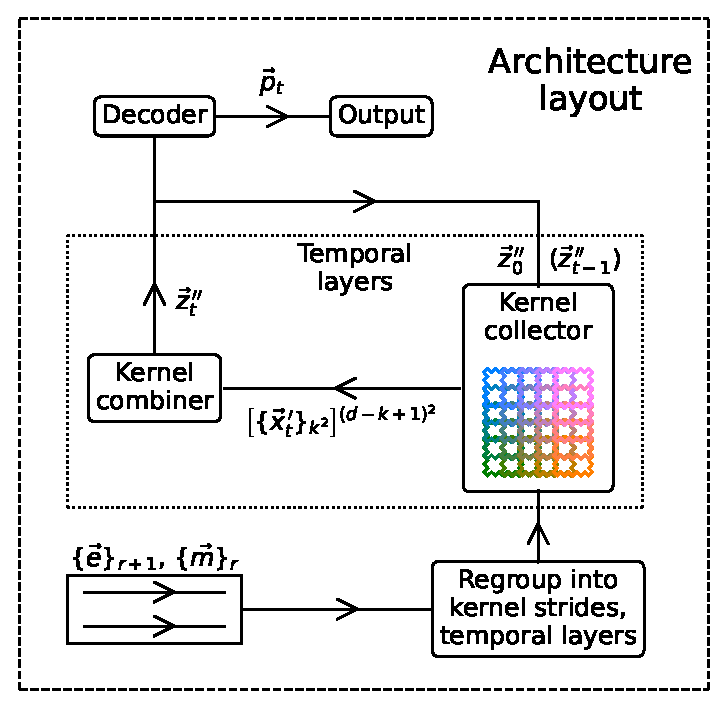
\includegraphics[width=0.9\textwidth]{general_architecture_layout.pdf}
\ccaption
{Layout of the compact RCNN architecture}
{
The inputs to the compact RCNN workflow are the stabilizer measurements from $r$ rounds, $\vec{m}$, and associated $r+1$ rounds of detector events, $\vec{e}$, which are displayed at the bottom left corner, with the vector notation representing qubit positions, and the subscripts in curly braces representing the temporal dimensionality.
The inputs are regrouped into kernels based on the spatial positions of the measure qubits and are fed sequentially into the layers of the NN, enclosed in dotted lines, that define the recurrent time evolution of the error state of the surface code. Each temporal layer consists of its own instances of a kernel collector, which is responsible for constructing the unique kernel types and traversing the entire surface code with them, and a kernel combiner, which is responsible for constructing a separate rule instance to combine the $x$-like evaluation results of the kernels (a list of $(d-k+1)^2$ number of $k^2$-dimensional vectors) into a $d^2$ array of $z$-like results. The output of the kernel combiner defines a multidimensional error state for the temporal slice and is fed into the next temporal slice as the last known (or initial) state. It can also be decoded through a decoder layer to produce a vector of probabilities for the logical observables of the circuit. As used throughout the paper, singly-primed variables denote the outputs of the kernels, and doubly-primed variables denote the outputs of the kernel combiner.
}
\label{fig:RCNN-layout}
\end{figure*}

%%%%%%%%%%%%%%%%%%%%%%%%%%%%%
\begin{figure*}[htb]
\centering
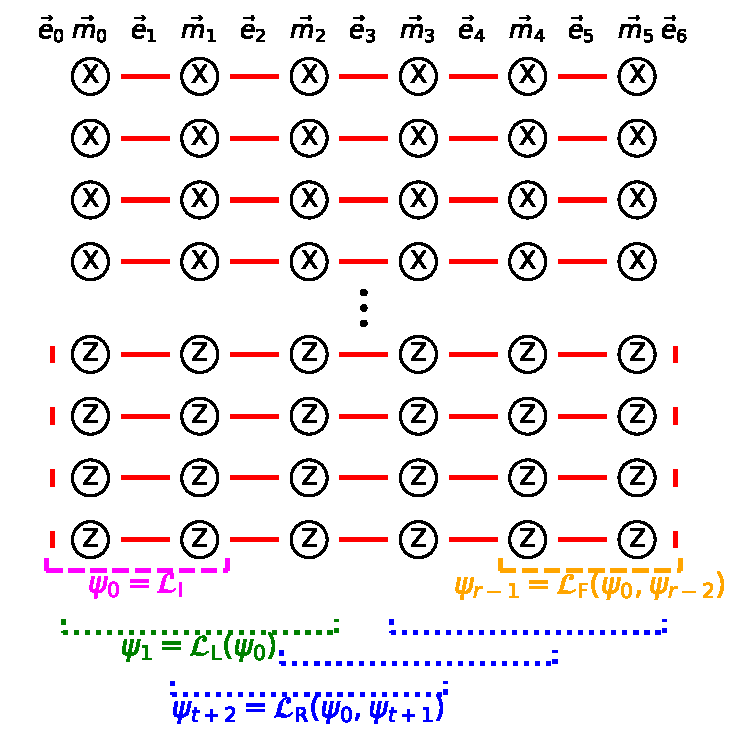
\includegraphics[width=0.9\textwidth]{RCNN_layer_progression_d3_r6.pdf}
\ccaption
{Layer progression in the recurrent NN architecture}
{
Illustrated is an example for a memory experiment over the logical $Z_L$ observable in an arbitrary distance-$d$ surface code with $r=6$ rounds. Each column of circles marks a different stabilizer measurement round, with the circles corresponding to the readings from the $X$ or $Z$ measure qubits, $\vec{m}_t$ for $0\leq t \leq r-1$. The horizontal red lines mark detector events that check for the consistency of measure qubit readings, $\vec{e}_t$ for $1 \leq t \leq r-1$, and the vertical red lines next to the $Z$ measure qubit readings mark the unique detector events associated with these readings at the beginning, $\vec{e}_0$, and end of the memory experiment, $\vec{e}_{r}$.
Each bracket at the bottom corresponds to a different pass in the recurrent architecture, with the extent of the brackets demarcating the measure qubit readings and detector events that are used as input features.
The initialization layer, $\mathcal{L}_I$ (magenta), provides an initial error state $\vec{z}^{\,\prime\prime}_0$ from $\vec{m}_0$, $\vec{m}_1$, $\vec{e}_0$, and $\vec{e}_1$.
The lead-in layer, $\mathcal{L}_L$ (green), updates the error state to $\vec{z}^{\,\prime\prime}_1$ using the first available triplet stabilizer state parametrization from $\vec{m}_{0 \text{---} 2}$, $\vec{e}_1$ and $\vec{e}_2$, and the state $\vec{z}^{\,\prime\prime}_0$.
The recurrent layer, $\mathcal{L}_R$ (blue), then strides through the rest of rounds one by one: To obtain each error state update $\vec{z}^{\,\prime\prime}_{t}$ ($t\geq2$), this layer uses the triplet stabilizer state parametrization from $\vec{m}_{(t-1) \text{---} (t+1)}$, $\vec{e}_{t}$ and $\vec{e}_{t+1}$, the previous error state $\vec{z}^{\,\prime\prime}_{t-1}$, and the initial error state $\vec{z}^{\,\prime\prime}_{0}$.
At the end, the finalization layer, $\mathcal{L}_F$ (orange), provides the final error state prediction $\vec{z}^{\,\prime\prime}_{r-1}$ upon receiving $\vec{m}_{r-2}$ and $\vec{m}_{r-1}$, $\vec{e}_{r-1}$ and $\vec{e}_r$, and the last known error state $\vec{z}^{\,\prime\prime}_{r-2}$ and the initial error state $\vec{z}^{\,\prime\prime}_{0}$.
}
\label{fig:RCNN-layer-prog}
\end{figure*}
%%%%%%%%%%%%%%%%%%%%%%%%%%%%%


The initial state kernel layer is the simplest in structure. As illustrated in Fig.~\ref{fig:RCNN-init-arch}, the stabilizer measurements and detector events are passed through stabilizer measurement and detector event embedders discussed in Section~\ref{sec:kernels-r2}, respectively. 
The quadratic representation of the inputs are then passed through separate dense layers with no bias and same output dimensions so that they can be added element-wise -- one should note that this approach is equivalent to having a single dense layer with no bias over the union of the outputs of the embedding layers. 
The final set of $z$-like pre-combination error states are exponentiated and passed into the combination step of the initial temporal layer.


%%%%%%%%%%%%%%%%%%%%%%%%%%%%%
\begin{figure*}[htb]
\centering
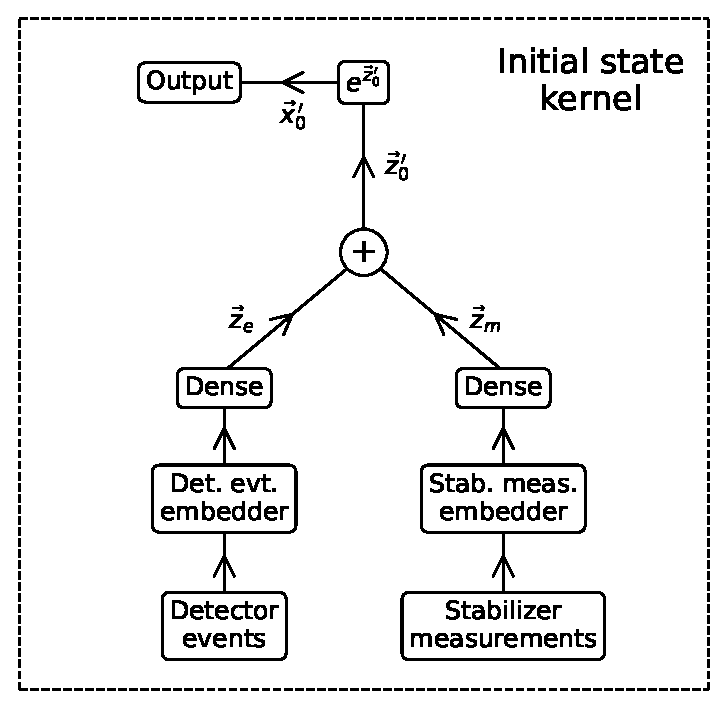
\includegraphics[width=0.6\textwidth]{initial_state_kernel_architecture.pdf}
\ccaption
{Initial state kernel architecture}
{
The detector events and stabilizer measurements that pertain to each kernel stride pass through embedder layers that convert linear or quadratic representations of the bits into values between -1 and 1.
The output of the embedders pass through dense layers with no bias term to convert them to $z$-like vectors of $k^2$ elements, and the two vectors are added. The final result of the kernel is returned as $x$-like values after element-wise exponentiation.
}
\label{fig:RCNN-init-arch}
\end{figure*}
%%%%%%%%%%%%%%%%%%%%%%%%%%%%%

As mentioned before, all kernel layers except the initial state kernel account for a set of prior states from the full temporal layer evaluation. This is accomplished through a state correlator layer architecture, illustrated in Fig.~\ref{fig:RCNN-state-corr}. The state correlator first converts the $z$-like input states from $n$ time steps, including the $z$-like states that result from the combination of dense layers in each kernel, into $n$ $\vec{\alpha}$-variables, $n-1$ $\vec{f}$-variables, and $n(n-1)/2$ $\vec{c}_\varphi$-variables. 
In this notation, the vector indices run over the data qubits of the kernel, and each of these sets of variables are determined through transformations of $z$-like underlying variables, parametrized linearly over the passed $z$-like states, with trainable weights initialized before training to 0, and trainable bias parameters initialized at 1. 
The $\alpha$-variables, bounded between -1 and 1, act as sign reversion indicators over the input states. 
After transforming the products $\vec{\alpha} \cdot \vec{z}$ using the exponential function into $x$-like values, we combine them using the $\vec{f}$ fractions and the $\vec{c}_\varphi$ phase factors in a way algebraically similar to the combination of kernel outputs described in Section~\ref{sec:kerncomb}. The final $x$-like outputs of the state correlator constitute the outputs of the kernel that maintains the correlator as well.


%%%%%%%%%%%%%%%%%%%%%%%%%%%%%
\begin{figure*}[htb]
\centering
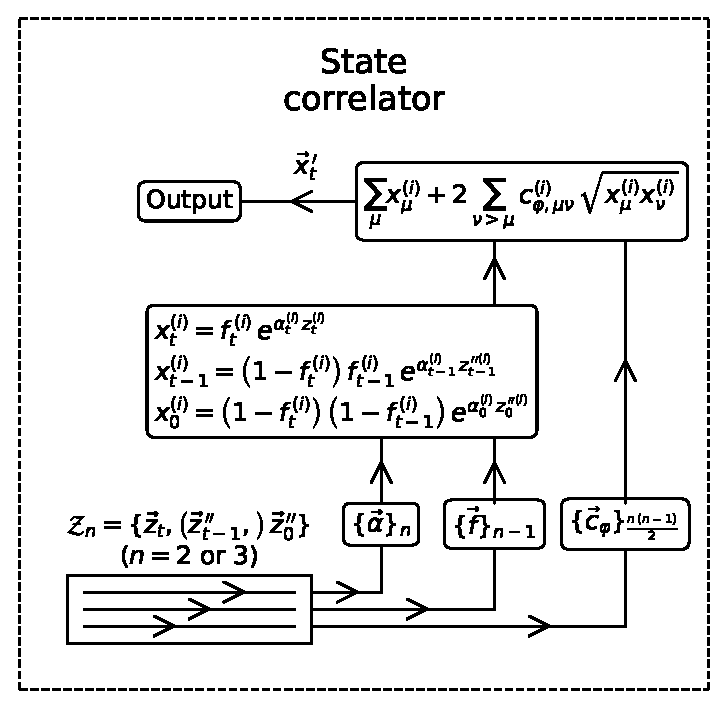
\includegraphics[width=0.6\textwidth]{state_correlator_architecture.pdf}
\ccaption
{State correlator architecture}
{
The inputs to the correlator are the kernel state prediction at current time, the state prediction from the initial temporal layer, and, if distinct from the initial state, the state prediction from the temporal layer for the previous round. 
For each input state, the values $\vec{\alpha}$ with $\abs{\alpha}<1$ are parametrized through a $\mathrm{tanh}(\vec{z}_\alpha)$ transformation such that $\vec{z}_\alpha$ depends linearly on the input states, along with a constant term. The set of $\vec{f}$ values that define recursive fractions for the states are also found in a similar way, but with a sigmoid transformation instead to keep the fractions bounded between 0 and 1. 
The phase terms $\vec{c}_\varphi$ between the states are constructed with a similar hyperbolic tangent transformation, independent of $\vec{\alpha}$. 
The vectors $\vec{\alpha}$ and $\vec{f}$ are used to compute $x$-like variables for each time step, with the sign of each $\alpha$ signifying whether the error probability that could be obtained by the corresponding state should be inverted or not. One can then combine the computed $x$-like variables as absolute values of complex numbers with phase differences using $\vec{c}_\varphi$ to obtain a final $x$-like vector. In the illustrated mathematical expressions, the superscript $(i)$ signifies element-wise operations, and the Greek-letter indices $\mu$ and $\nu$ are used in the $x$-like variable summation over the time steps.
}
\label{fig:RCNN-state-corr}
\end{figure*}
%%%%%%%%%%%%%%%%%%%%%%%%%%%%%


Because they feature state correlator layers, the lead-in, recurrent, and final state kernels are structurally similar to each other. 
The flowcharts of the lead-in and recurrent kernel layers are displayed in Fig.~\ref{fig:RCNN-lirec-arch}, whereas that of the final state kernel is displayed in Fig.~\ref{fig:RCNN-final-arch}.
The only differences between the base class of the lead-in and recurrent state kernels, and the class for the final state kernel, are the number of rounds processed as input, and the fact that the special detector events at the end of the full QEC cycle are also passed to the final state kernels.
These differences lead to the choices to utilize the triplet state probability embedder layer in lead-in and recurrent layers, and the stabilizer measurement embedder layer in the final state kernel for the quadratic representation of the stabilizer measurements.


%%%%%%%%%%%%%%%%%%%%%%%%%%%%%
\begin{figure*}[htb]
\centering
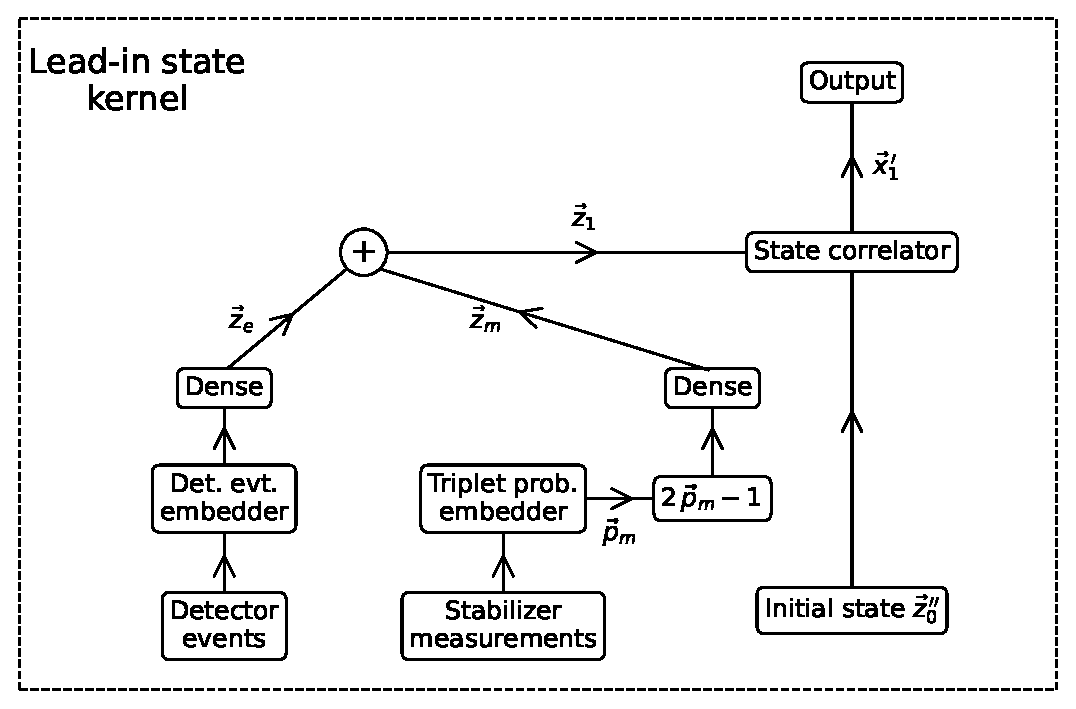
\includegraphics[width=0.9\textwidth]{leadin_state_kernel_architecture.pdf}\\
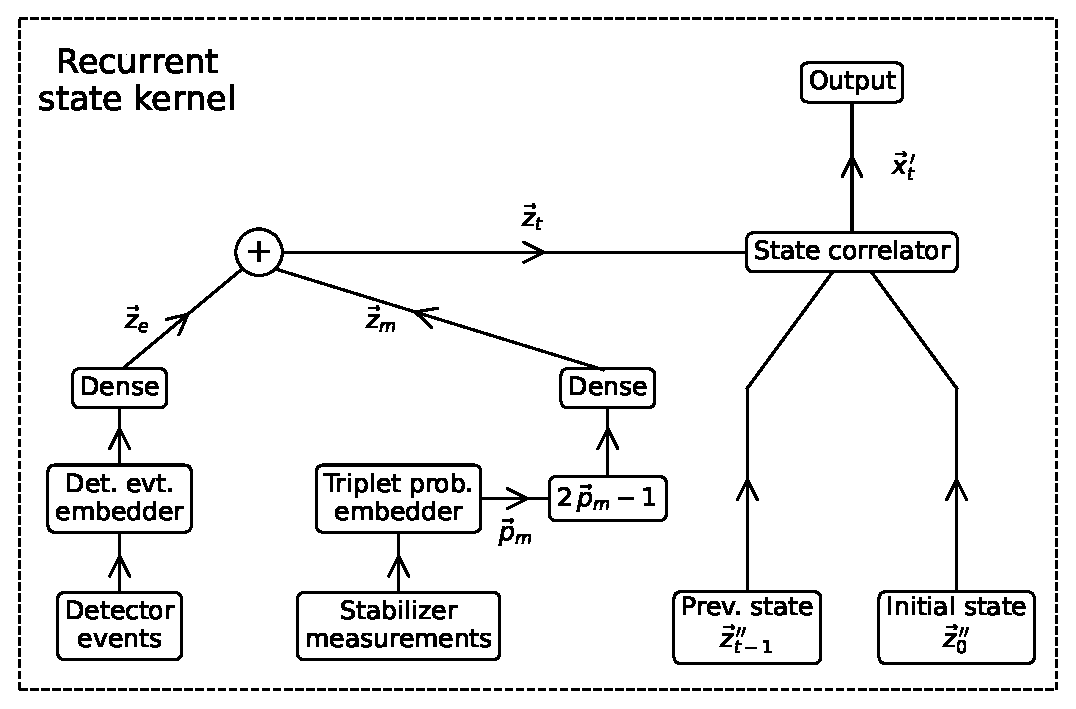
\includegraphics[width=0.9\textwidth]{recurrent_state_kernel_architecture.pdf}
\ccaption
{Lead-in and recurrent state kernel architectures}
{
Lead-in state kernel, top: The detector events that pertain to each kernel stride pass through an embedder layer that converts linear or quadratic representations of the bits into values between -1 and 1, and these values are then passed through a dense layer with no bias term. Similarly, stabilizer measurements are passed through a triplet stat probability embedder, and the probabilities are transformed linearly into values between -1 and 1 before passing through a similar dense layer.
The $z$-like results of the two dense layers, each being vectors of $k^2$ elements, are summed, and together with the initial states of the data qubits corresponding to the kernel window, they are passed to a state correlator. The correlator produces the final $x$-like output of the lead-in layer.
Recurrent state kernel, bottom: The architecture is almost exactly the same as that of the lead-in state. The only difference is that the recurrent state kernel passes both the previous and the initial state of the data qubits within the kernel window to the state correlator.
}
\label{fig:RCNN-lirec-arch}
\end{figure*}
%%%%%%%%%%%%%%%%%%%%%%%%%%%%%



%%%%%%%%%%%%%%%%%%%%%%%%%%%%%
\begin{figure*}[htb]
\centering
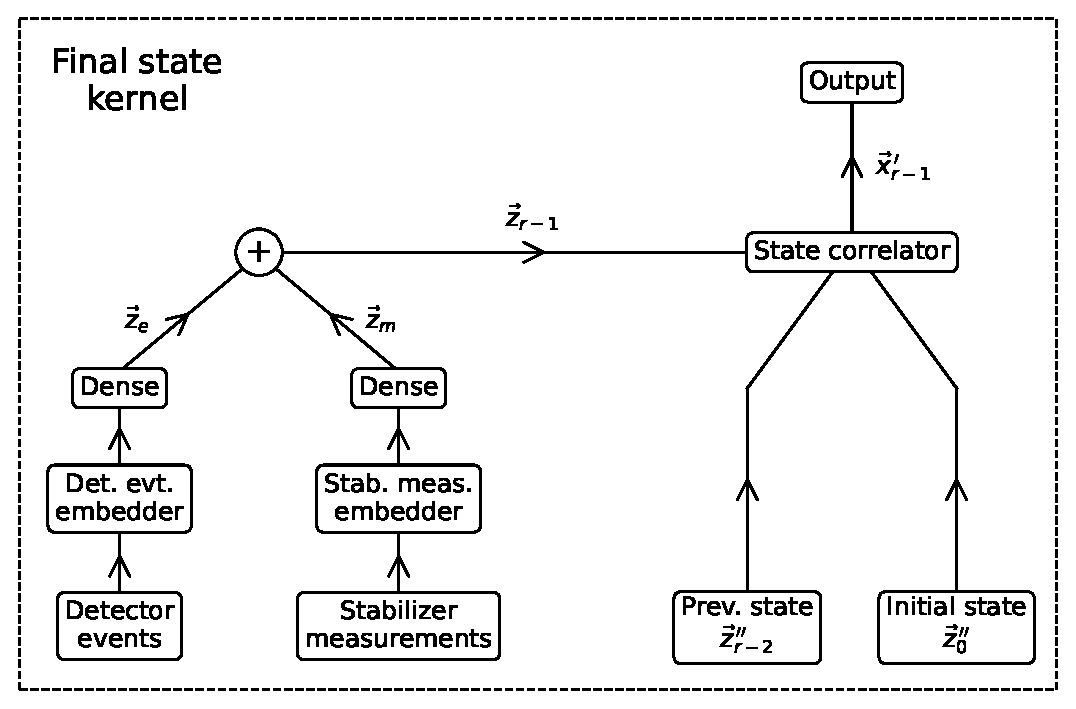
\includegraphics[width=0.9\textwidth]{final_state_kernel_architecture.pdf}
\ccaption
{Final state kernel architectures}
{
The detector events and stabilizer measurements that pertain to each kernel stride pass through embedder layers that convert linear or quadratic representations of the bits into values between -1 and 1.
The output of the embedders pass through dense layers with no bias term to convert them to $z$-like vectors of $k^2$ elements, and the two vectors are added.
Together with the initial and last states of the data qubits corresponding to the kernel window, the summed vector is passed to a state correlator, and the correlator produces the final $x$-like output of this layer.
When there are only two rounds in a QEC cycle, the initial and last states are identical, so the implementation passes only one prior state.
}
\label{fig:RCNN-final-arch}
\end{figure*}
%%%%%%%%%%%%%%%%%%%%%%%%%%%%%


In determining the final probability of logical observable errors, the architecture provides the option to run in two different modes:
\begin{itemize}
\item In standard mode, the architecture determines a probability value for either all rounds requested, or a certain number of specified rounds, including the last round. If a valid cutoff round is specified, even if it is the last round, we define this prediction as an early stopping condition and do not run the final temporal layer. 
Otherwise, the predictions are produced after adding the final temporal layer.
\item In per-round prediction mode, the architecture determines a probability value for each round in the QEC cycle except for the first one, which is consumed by the initial temporal layer for reliable warmup without any corresponding output. This option is useful if one would like to train the NN over a shorter cycle that covers each temporal layer and reuse it for longer ones.
\end{itemize}
Ultimately, the specific use case would dictate how the architecture is trained and utilized, so we leave it to the user to decide which mode suits their needs best.


\section{Summary and outlook}

Neural networks are promising error decoders for quantum circuits, providing the promise to learn complex qubit readout parameters and error patterns that are difficult to quantify experimentally, or algebraically through non-NN approaches.
In order to limit the duration of quantum error correction cycles to $\ll 1\mus$, these NNs need to run on hardware acceleration devices such as FPGAs, GPUs, and other specialized ASICs. The state-of-the-art FPGAs can typically accept only $\Order(100,000)$ parameters, and the development of specialized ASICs will likely face similar limits. For this reason, large NNs currently require a more involved room-temperature computational support system, which would increase the costs to make quantum computing systems commercially available.

The primary goal of this paper is to design a compact decoder NN architecture to maximize the number of NN parameters shared and keep the parameter count within the limits of a typical FPGA. The key novel feature of our architecture is the accounting of the spatial symmetries of the surface code in a recurrent structure, and using minimal additional features, we have achieved decoding performance that is competitive with the MWPM-based PyMatching~\cite{Higgott:2023} algorithm while only requiring $\leq72917$ NN parameters.

Since our primary focus has been to find a method to account for the rotational and translational symmetries, we leave a more thorough implementation of accounting for nonuniformities in hardware noise to a future study, providing only a simplistic option in our architecture, as mentioned in Section~\ref{sec:kerncomb}. Some of the mathematical formulations explored in this architecture may also need to be modified in order to improve decoder performance over larger $d$ or $r$ values.

An anticipated area of investigation for the further development of the presented architecture is the inclusion of additional error-sensitive data from qubit readout, \eg, I-Q information as exemplified in Ref.~\cite{Bausch:2023jgi}. In this context, one could also consider in the farther future joint error correction and mitigation schemes, \eg, as conceptually explored in Ref.~\cite{Sarica:2023}.

Since our NN architecture is currently based on the TensorFlow Python API, which is a general NN framework not adequately optimized for the fast execution times required in QEC cycles, another future development stage would be to re-code the architecture using basic C/C++ for optimized implementation in FPGAs and other room-temperature hardware acceleration devices, through \textsc{hls4ml}~\cite{hls4ml} or other language synthesis frameworks.




\bibliographystyle{JHEP}
\bibliography{main.bib}


\end{document}
